\documentclass[a4paper,10pt]{beamer}
\usepackage[utf8x]{inputenc}
\usepackage[T1]{fontenc}
\usepackage[french]{babel}
\usepackage{hyperref,graphicx,multicol,eurosym,tabularx,color}
\usetheme{Berkeley}
\setbeamercolor{structure}{fg=cyan!60!black}
\setbeamertemplate{navigation symbols}{\large \insertframenumber /\inserttotalframenumber}
\newcolumntype{M}[1]{>{\centering\arraybackslash}m{#1}}

\title{Création d'objets 3D à partir de dessins 2D}
\author[Groupe 3INFO]{Aurélien Fontaine, Manutea Huang,
\\ Etienne Geantet, Arnaud Martin}
\institute[INSA de Rennes]{Institut National des Sciences Appliquées de Rennes}
\date{\today}

\begin{document}
	
	\begin{frame}
		\begin{titlepage}
			\centerline{
\includegraphics[scale=0.1]{images/logos/logoINSA.jpg}}
			\centerline{Encadrants : François Lehericey and Bertrand Coüasnon}	
		\end{titlepage}
	\end{frame}
	
	\section{Introduction}
	
	\begin{frame}{Introduction}
		\begin{itemize}
		\item Un projet proposé par les chercheurs de l'Irisa.
		\end{itemize}
		\centerline{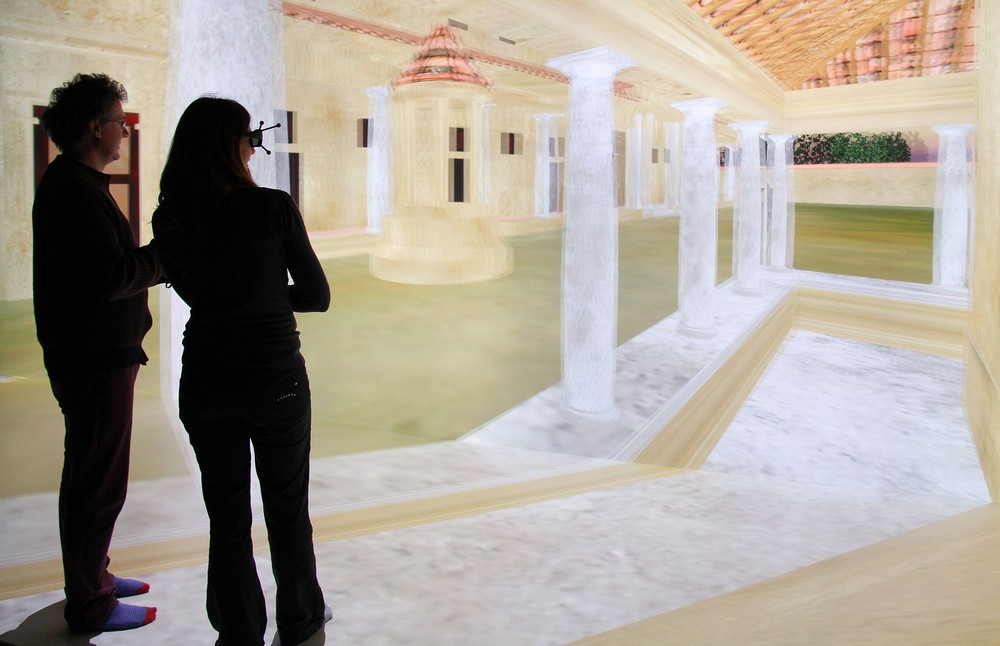
\includegraphics[scale=0.25]{images/intro/Immersia.jpg}}
		\centerline{Comment meubler rapidement une scène de réalité}
		\centerline{virtuelle avec divers objets 3D ?}
	\end{frame}
	
	\begin{frame}{Introduction}
		Pour l'étude du comportement physique des modèles 3D dans une scène, les chercheurs souhaitent pouvoir créer des objets rapidement.
		
		
		\begin{itemize}
			\item Ce projet a pour but de permettre la \textbf{création rapide} d'objets simples.
			\centerline{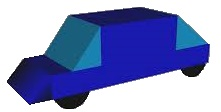
\includegraphics[scale=0.5]{images/intro/car.jpg}}
			\item L'application met l'accent sur la \textbf{simplicité} d'utilisation et \textbf{l'ergonomie}.
		\end{itemize}
		
	\end{frame}
	
	\begin{frame}{Sommaire}
		\tableofcontents
	\end{frame}
	
	\section{Cahier des charges}
	
	\begin{frame}{Cahier des charges}
		Notre projet doit respecter les contraintes suivantes:
		\begin{itemize}
			\item Cette application doit fonctionner sur tablette.
			\item Permettre la création d'objets 3D grâce à une suite de dessins à main levée.
			\item L'utilisateur disposera de plusieurs outils de dessin, afin de varier ses créations.
			\item L'application doit rester ergonomique, et utilisable intuitivement par tous.
			\item L'objet créé doit pouvoir être exporté vers un serveur Unity.
		\end{itemize}
	\end{frame}
	
	\section{Etat de l'art}
	
	\begin{frame}{Quelle technologie utiliser ?}
		
		\centerline{
\includegraphics[height=75pt]{images/techno/unity-logo.png}
			
\includegraphics[height=75pt]{images/techno/UE3_logo.png}
			
\includegraphics[height=75pt]{images/techno/CryENGINE3-Logo.png}}
		
		\centerline{
\includegraphics[height=75pt]{images/techno/opengl-logo.jpg}
			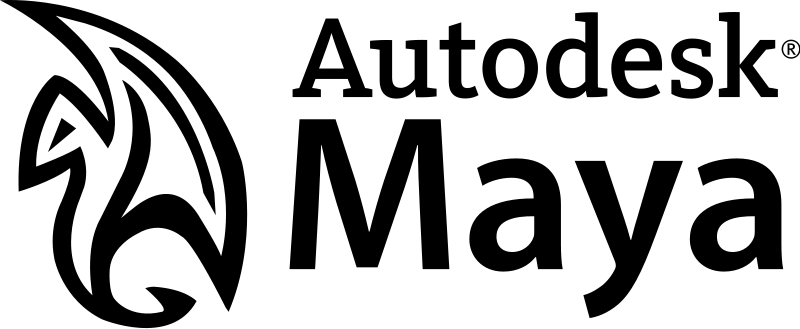
\includegraphics[height=60pt]{images/techno/auto.png}}
	\end{frame}
	
		\begin{frame}{Un comparatif}
			\begin{tabular}{|M{45pt}|M{40pt}|M{45pt}|M{75pt}|M{30pt}|}
				\hline
				\textbf{Software} & \textbf{Facile à apprendre} & \textbf{Manipule de nombreux objets} & \textbf{Prix} & \textbf{Aide pour tablettes}\\
				\hline
				\textit{Unreal Engine} & \color{green}{\checkmark} & \color{green}{\checkmark} & \color{orange}{19\euro/mois} + 5 \% & \color{red}{$\times$}\\
				\hline
				\textit{CryEngine} & \color{green}{\checkmark} & \color{green}{\checkmark} & \color{orange}{9.99\euro/mois} & \color{orange}{$\sim$}\\
				\hline
				\textit{OpenGl} & \color{red}{$\times$} & \color{orange}{$\sim$} & \color{green}{0\euro} & \color{red}{$\times$}\\
				\hline
				\textit{Autodesk Maya} & \color{red}{$\times$} & \color{green}{\checkmark} & \color{red}{\$185.00/mois} & \color{orange}{$\sim$}\\
				\hline
				\textit{Unity} & \color{green}{\checkmark} & \color{green}{\checkmark} & \color{green}{0\euro : licence gratuite} & \color{green}{\checkmark} \\
				\hline
			\end{tabular}
		\end{frame}
		
		\begin{frame}{Le petit plus pour Unity}
			\centerline{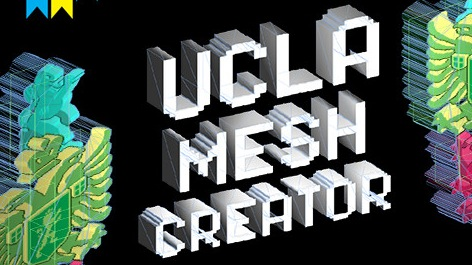
\includegraphics[height=80pt]{images/techno/ucla.jpg}}
			
			\begin{itemize}
				\item UCLA Mesh Creator : Une aide à la création d'objets en 3D à partir d'une texture
				\item Gros avantage : Réutilisable facilement et sans contrainte
			\end{itemize}
			
		\end{frame}
		

	
	\section{Conception}	
		\begin{frame}{Conception}
	 		En parallèle du choix de technologie, nous avons dû réfléchir en nous basant sur deux points centraux:
		
			\begin{itemize}
				  \item Définir comment être ergonomique : découper pas à pas pour s'assurer de la simplicité à chaque instant
				  \item Diviser le logiciel en éléments les plus simples possibles et indépendants pour organiser le développement
			\end{itemize}
		\end{frame}
		
		
		\begin{frame}{Comment être ergonomique?}
				Repérage des parties pouvant posé problèmes:
				
				\begin{itemize}
					\item Comment dessiner?
					\item Comment extruder ce dessin?
					\item Comment placer la figure créée dans l'environnement 3D?
					\item Comment se repérer dans notre création?
				\end{itemize}
		\end{frame}	
		
		\begin{frame}{Comment être ergonomique?}

				Comment dessiner?
					\begin{itemize}
						\item Interface sobre
						\item Menu d'outils déroulant
					\end{itemize}
				
				\centerline{
\includegraphics[scale=0.3]{images/Nono/img1.png}} \centerline{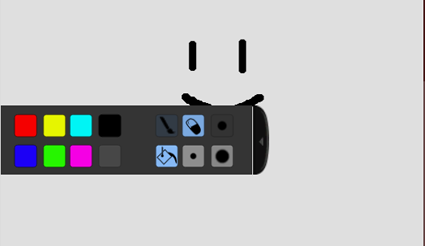
\includegraphics[scale=0.3]{images/Nono/img2.png}}
			


		\end{frame}	
		
		\begin{frame}{Comment être ergonomique?}
			
			Comment extruder ce dessin?
			\begin{itemize}
				\item Jeu d'icônes assez clair
				\item Limiter les options
				\item L'utilisateur n'a pas à intervenir plus que nécessaire
			\end{itemize}
			
			\centerline{
\includegraphics[scale=0.5]{images/Nono/img3.png}} 
			
			
			
		\end{frame}	
			
		\begin{frame}{Comment être ergonomique?}
						
				Comment placer la figure créée dans l'environnement 3D?
				
				\begin{itemize}
					\item Découper en plusieurs étapes
					\item Menu clair
					\item Ne pas surcharger d'informations
				\end{itemize}
				
				\centerline{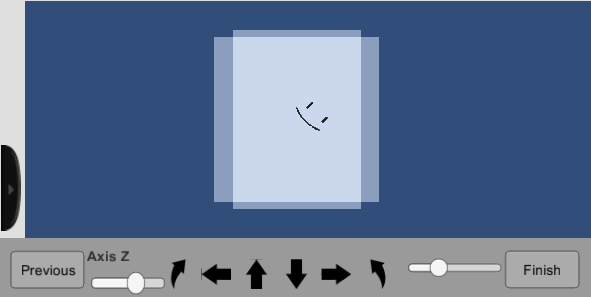
\includegraphics[scale=0.5]{images/Nono/img4.png}} 
						
						
						
		\end{frame}	
		
		\begin{frame}{Comment être ergonomique?}
			
			Comment se repérer dans notre création?
			
			\begin{itemize}
				\item Vue d'ensemble permanente
				\item Caméra mobile
				\item Limiter les déplacements
			\end{itemize}
			
			\centerline{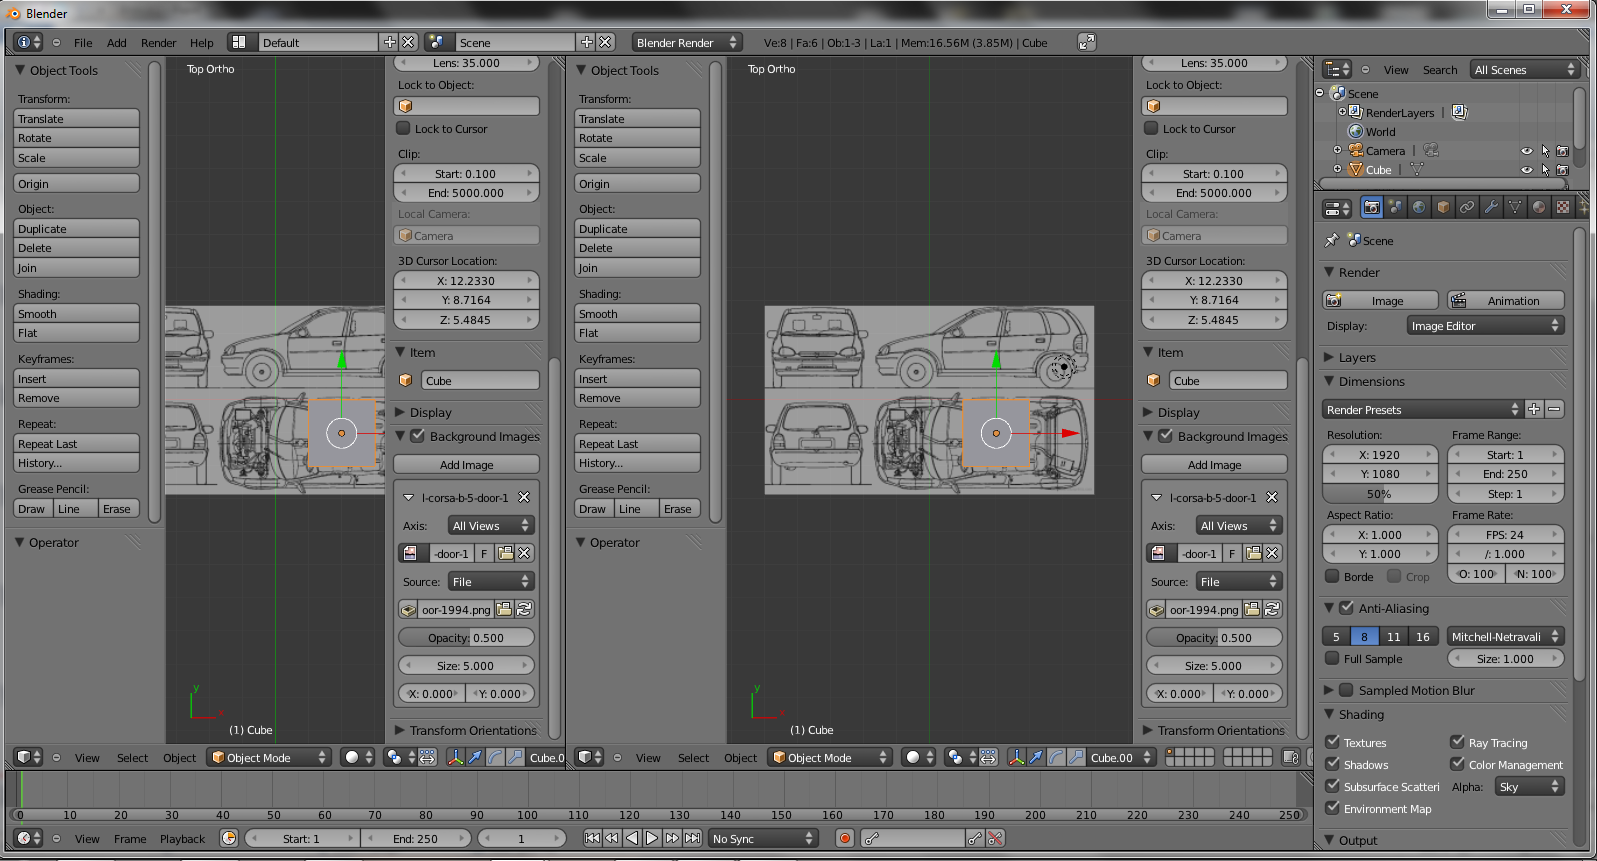
\includegraphics[scale=0.5]{images/Nono/img5.png}} 
			
			
			
		\end{frame}	
	\begin{frame}{Architecture logicielle} %Découpage de l'application}
		\huge Comment découper l'application?
	\end{frame}
	
	\begin{frame}{Architecture logicielle} %Découpage de l'application}
		%Archi logi Manutea
		\centerline{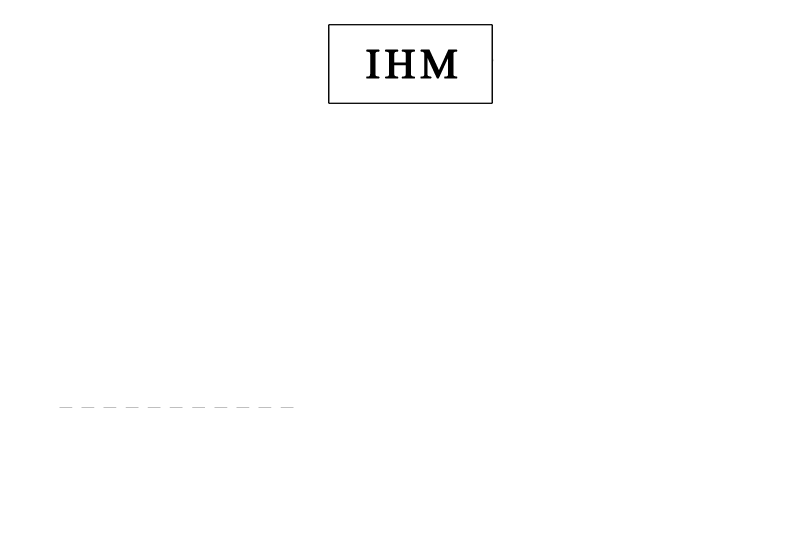
\includegraphics[scale=0.3]{images/archilogi/archi1.png}}
	\end{frame}
	\begin{frame}{Architecture logicielle} %Découpage de l'application}
		%Archi logi Manutea
		\centerline{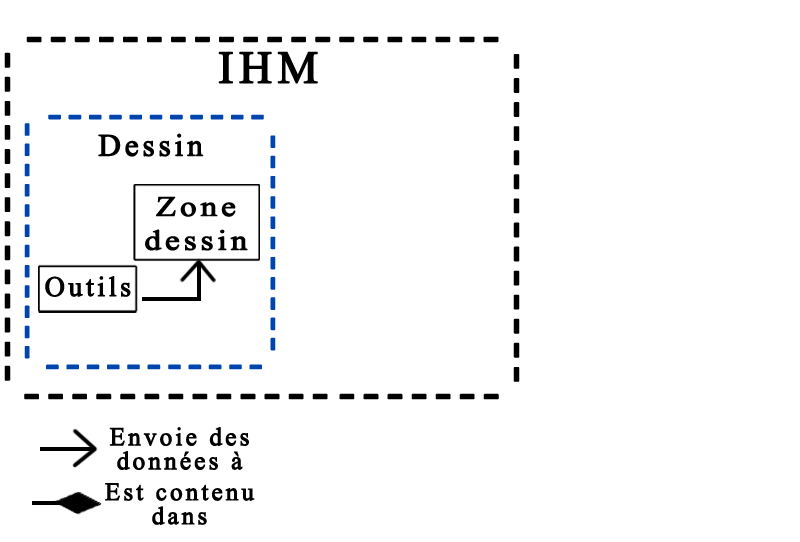
\includegraphics[scale=0.3]{images/archilogi/archi2.png}}
	\end{frame}
	\begin{frame}{Architecture logicielle} %Découpage de l'application}
		%Archi logi Manutea
		\centerline{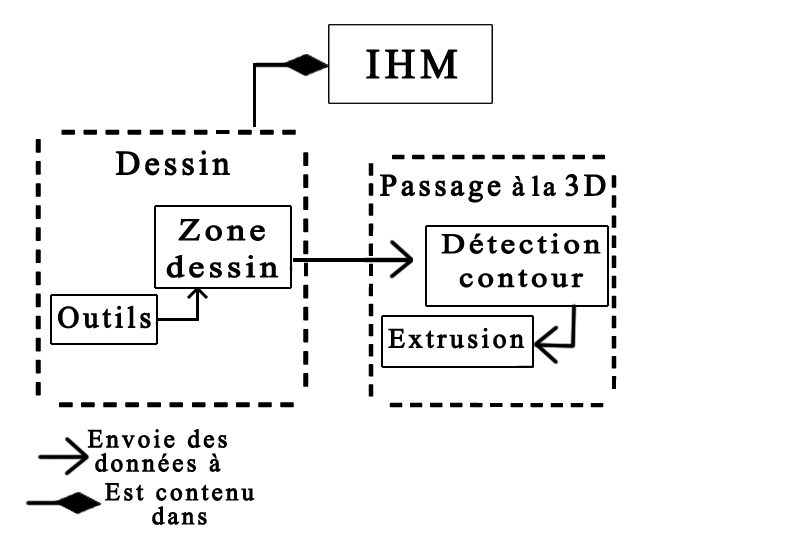
\includegraphics[scale=0.3]{images/archilogi/archi3.png}}
	\end{frame}
	\begin{frame}{Architecture logicielle} %Découpage de l'application}
		%Archi logi Manutea
		\centerline{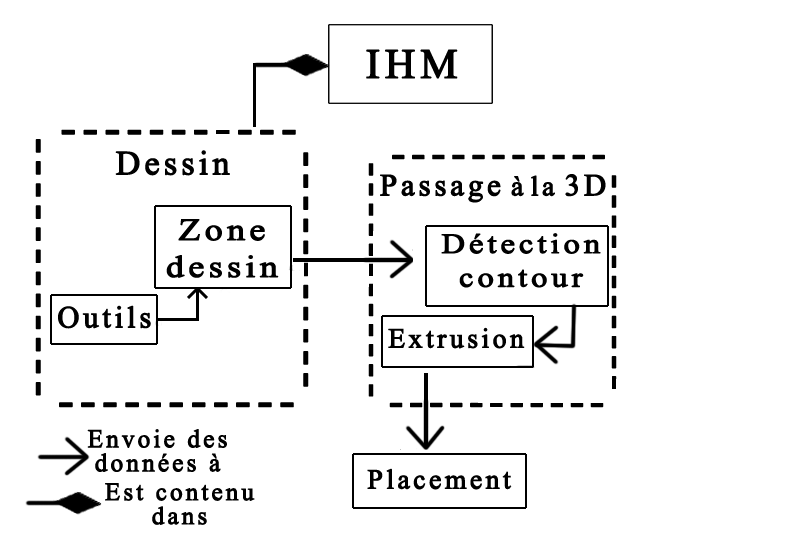
\includegraphics[scale=0.3]{images/archilogi/archi4.png}}
	\end{frame}
	\begin{frame}{Architecture logicielle} %Découpage de l'application}
		%Archi logi Manutea
		\centerline{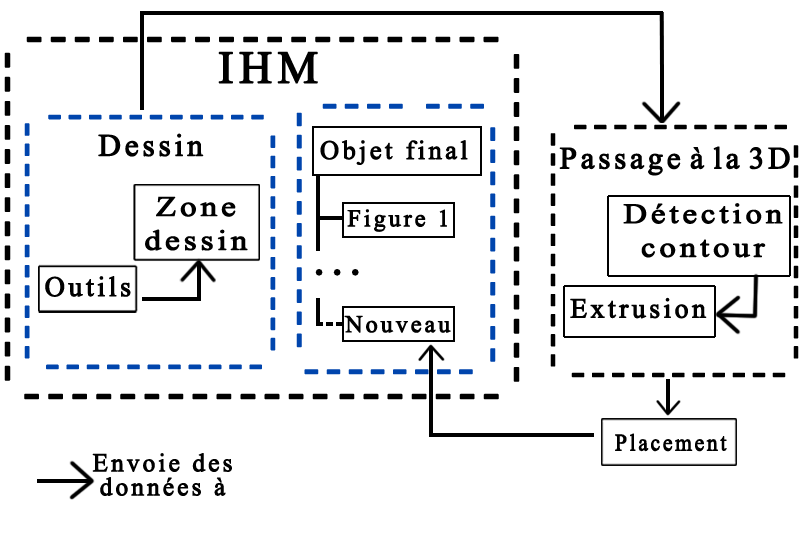
\includegraphics[scale=0.3]{images/archilogi/archi5.png}}
	\end{frame}	
	\begin{frame}{Architecture logicielle} %Découpage de l'application}
		%Archi logi Manutea
		\centerline{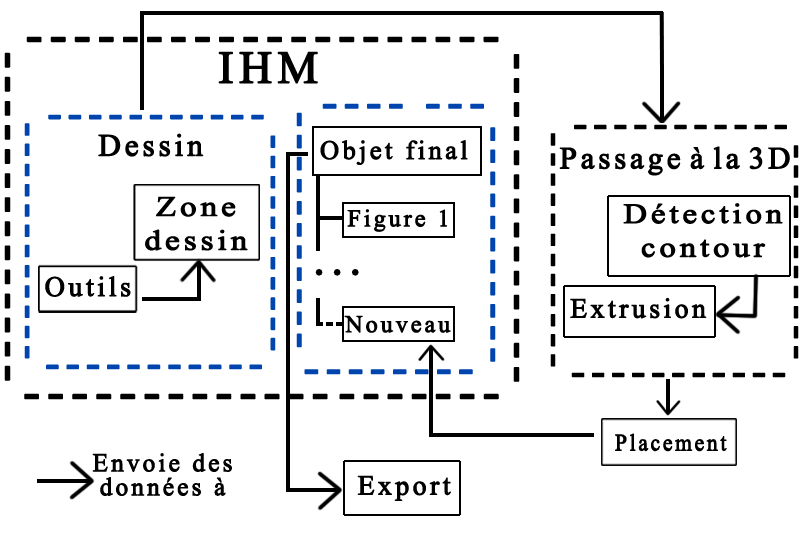
\includegraphics[scale=0.3]{images/archilogi/archi6.png}}
	\end{frame}
			
	\section{Etape par étape}
		%Expliquer nos choix par rapports aux objectifs énoncés
			\begin{frame}{Etape par étape}
				Ce qui a été fait:
					\begin{itemize}
						\item Choix technologique : Unity
						\item Définition du fonctionnement de l'application
						\item L'architecture du logiciel
					\end{itemize}
				Grâce tout cela, nous avons les éléments pour développer l'application.
			\end{frame}
		
		
	\begin{frame}{IHM}
			Problématique:
				\begin{itemize}
					\item Accueillir les éléments définis précédemment
					\item Simple
				\end{itemize}
				
			Solution:
				\begin{itemize}
					\item Technologie: utilisation du système d'UI (outils de menus et fenêtre) d'Unity
					\item Des espaces prêt à accueillir les autres composants
				\end{itemize}
				\centerline{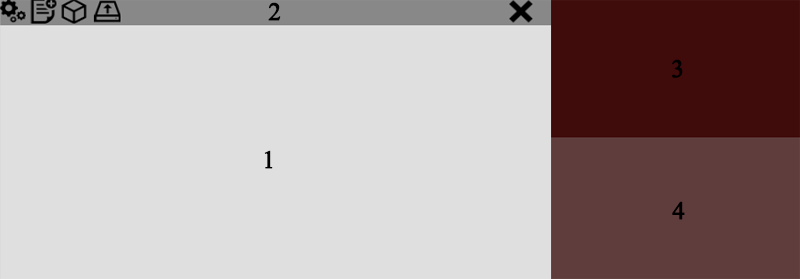
\includegraphics[scale=0.3]{images/Nono/img6.png}} 
	\end{frame}
	
	\begin{frame}{Menu d'outils}
		Pour assurer l'ergonomie et l'évolution de ce menu:
			\begin{itemize}
				\item Choix de couleur limité
				\item Choix de taille limité
				\item Choix d'outils limité
					\centerline{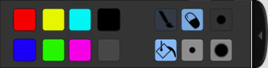
\includegraphics[scale=0.4]{images/Nono/img7.png}} 
				\item Modèle de fonction simple
							\centerline{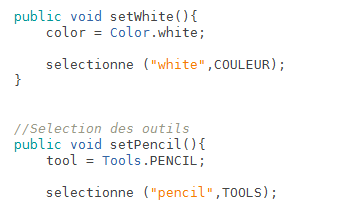
\includegraphics[scale=0.6]{images/Nono/img8.png}} 
			\end{itemize}


	\end{frame}
	
	\begin{frame}{La zone de dessin}
		Le dessin doit apparaître sur la texture de l'objet.
			\centerline{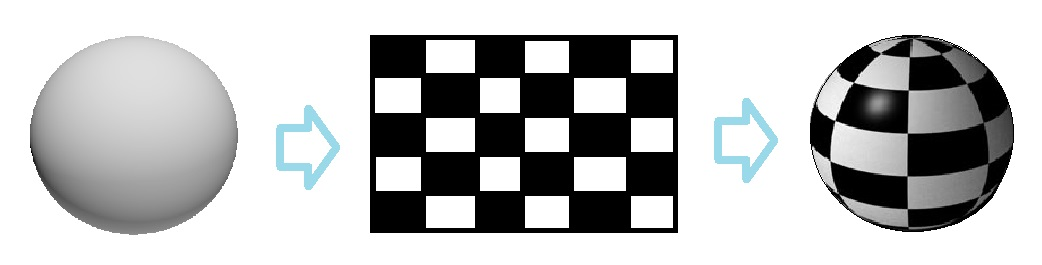
\includegraphics[scale=0.4]{images/intro/spheres.jpg}}
			
			\begin{itemize}
				\item Les plan (GameObject dans Unity) et la texture n'ont pas le même référentiel. 
				\item Pour accéder au pixel sur lequel on clic, on doit chercher le point d'intersection entre un Ray que l'on projette, et la zone de dessin.
				\item Le dessin se fait simplement en modifiant la texture aux endroit où  l'on clique.
			\end{itemize} 
		La fond de la texture doit être en alpha pour n'extruder que ce qui a été colorié.
	\end{frame}
	
	\begin{frame}{La zone de dessin}
		\begin{itemize}
		\item Unity va tester la position du doigt à chaque frame.
		Pour garder un tracé continu, on trace la droite entre le point courant et le dernier point.
		\centerline{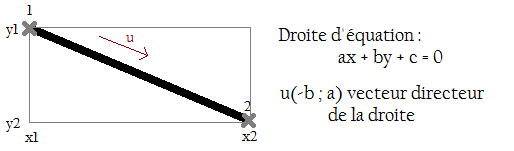
\includegraphics[scale=0.4]{images/intro/trait.png}}
		
		\item Pour le remplissage de la texture avec l'outil Bucket, on a utilisé un algorithme de remplissage par pile explicite.
	\end{itemize}
	\end{frame}
	
	\begin{frame}{L'extrusion}
		Plusieurs étapes pour passer d'une texture à un objet :
		\begin{itemize}
			\item Détection des contours du dessin
			\item Création de meshes
			\item Assemblage des meshes -> Objet 3D
			\item Application de la texture pour rendre l'objet coloré
		\end{itemize}
		
		L'utilisation de UCLA Mesh Creator nous a facilité dans le développement, notamment au niveau de la détection des contours et de l'assemblage des meshes.
	\end{frame}
		
	
	\begin{frame}{Placement}
			Modèle défini précédemment:
					\centerline{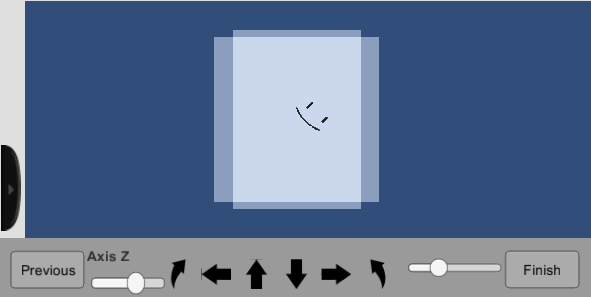
\includegraphics[scale=0.4]{images/Nono/img4.png}} 
					Il faut:
			\begin{itemize}
				\item Une caméra de suivi changeant d'axe à chaque étape.
				\item Des boutons pour déplacer l'objet.
				\item Pouvoir modifier la taille de l'objet. Choix retenu : taille globale et taille selon un axe.
				\item Rendre les autres objets légèrement transparents lors du placement.

			\end{itemize}
					
	\end{frame}
	
	
	\begin{frame}{Envoi des données}
		\centerline{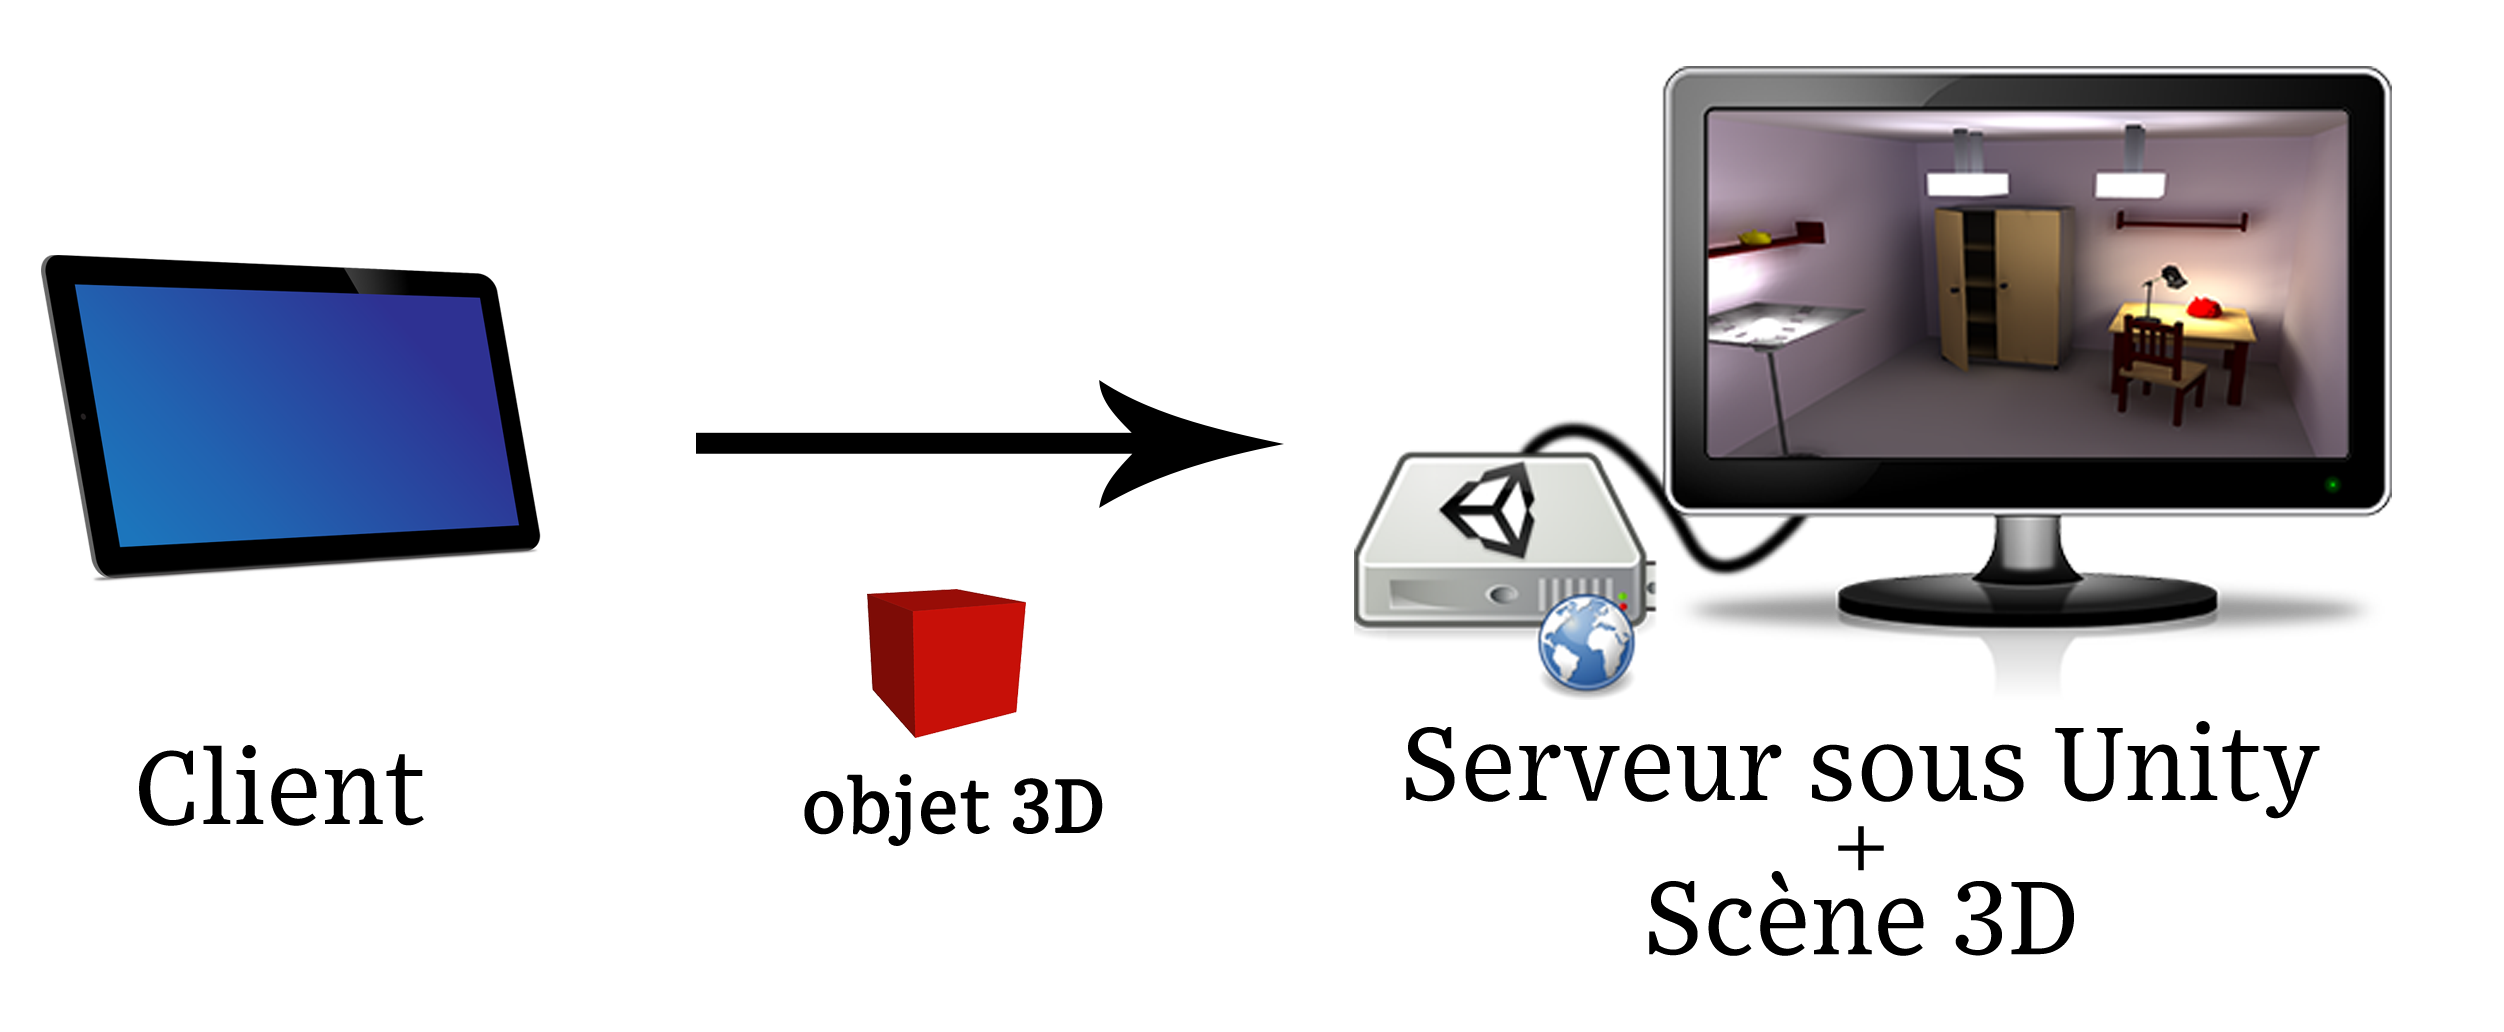
\includegraphics[height=120pt]{images/network/sending_model2.png}}
	\end{frame}
	
	
	\begin{frame}{Côté serveur}
		\centerline{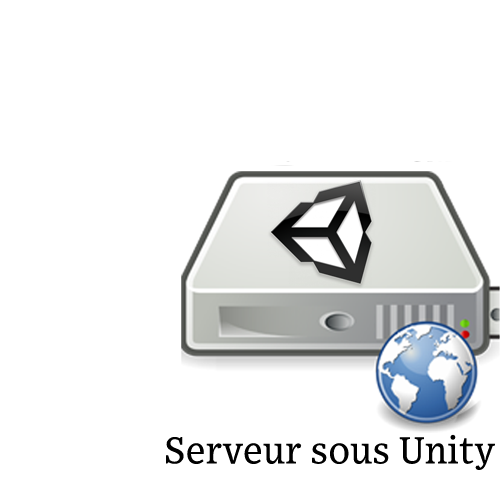
\includegraphics[height=150pt]{images/network/plugin1.png}}
		\invisible{
		\begin{itemize}	
			\item  Léger 
			\item Reçoit les données 
			\item Intégré dans la scène 3D
			\item Affiche l'objet 
		\end{itemize}	}
		
	\end{frame}
	\begin{frame}{Côté serveur}
		\centerline{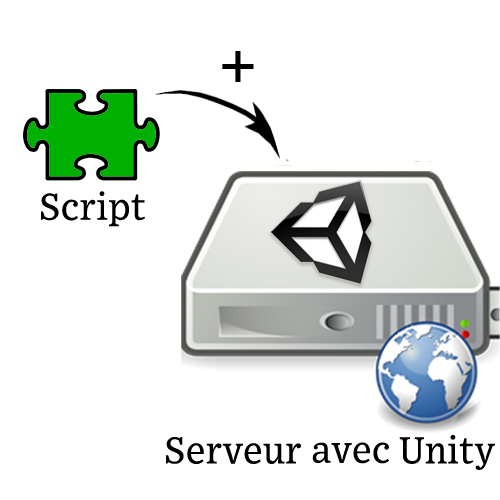
\includegraphics[height=150pt]{images/network/plugin.png}}
		\begin{itemize}	
			\item \pause Léger \pause
			\item Reçoit les données \pause
			\item Affiche l'objet 
		\end{itemize}	
		
	\end{frame}
	
	
	\begin{frame}{Socket TCP}
				\centerline{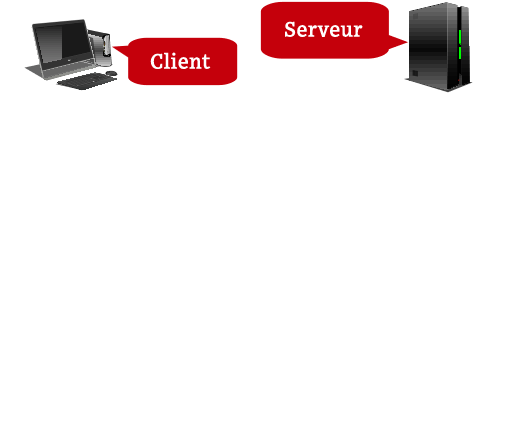
\includegraphics[height=150pt]{images/network/tcp-socket1.png}}
				\invisible{
					\begin{itemize}
						\item Dispose de classes prévues à cet effet en C\#
						\item Documentée en C\# par Microsoft
						\item Permet d'envoyer des octets, donc flexible
					\end{itemize}
				}
	\end{frame}
	
	\begin{frame}{Socket TCP}
		\centerline{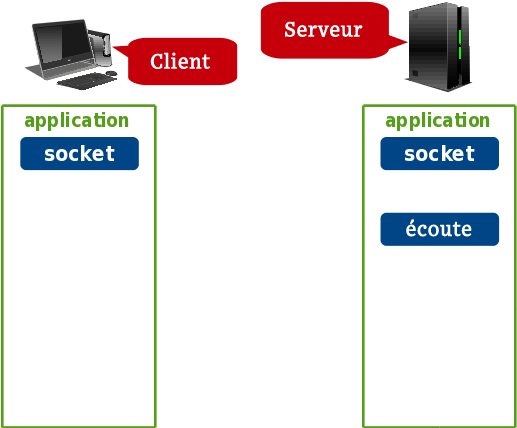
\includegraphics[height=150pt]{images/network/tcp-socket2.png}}
		\invisible{
			\begin{itemize}
				\item Dispose de classes prévues à cet effet en C\#
				\item Documentée en C\# par Microsoft
				\item Permet d'envoyer des octets, donc flexible
			\end{itemize}
		}
	\end{frame}
	\begin{frame}{Socket TCP}
		\centerline{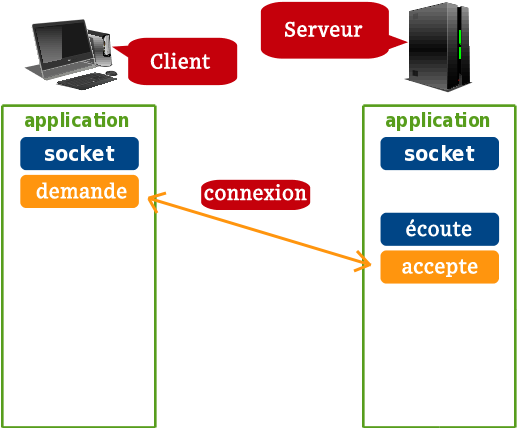
\includegraphics[height=150pt]{images/network/tcp-socket3.png}}
		\invisible{
			\begin{itemize}
				\item Dispose de classes prévues à cet effet en C\#
				\item Documentée en C\# par Microsoft
				\item Permet d'envoyer des octets, donc flexible
			\end{itemize}
		}
	\end{frame}
	\begin{frame}{Socket TCP}
		\centerline{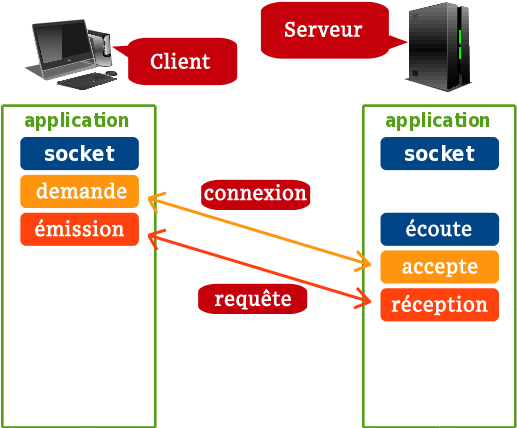
\includegraphics[height=150pt]{images/network/tcp-socket4.png}}
		\invisible{
			\begin{itemize}
				\item Dispose de classes prévues à cet effet en C\#
				\item Documentée en C\# par Microsoft
				\item Permet d'envoyer des octets, donc flexible
			\end{itemize}
		}
	\end{frame}
	\begin{frame}{Socket TCP}
		\centerline{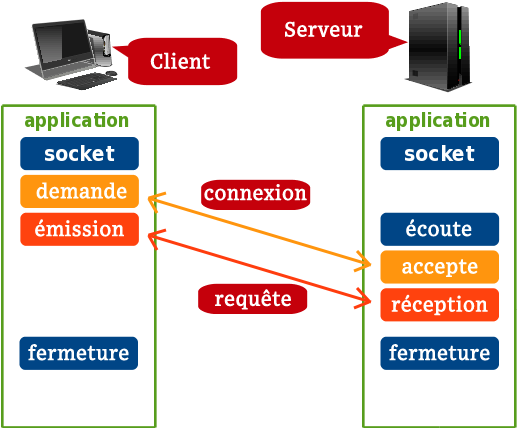
\includegraphics[height=150pt]{images/network/tcp-socket5.png}}
		\invisible{
			\begin{itemize}
				\item Dispose de classes prévues à cet effet en C\#
				\item Documentée en C\# par Microsoft
				\item Permet d'envoyer des octets, donc flexible
			\end{itemize}
		}
	\end{frame}
	\begin{frame}{Socket TCP}
		\centerline{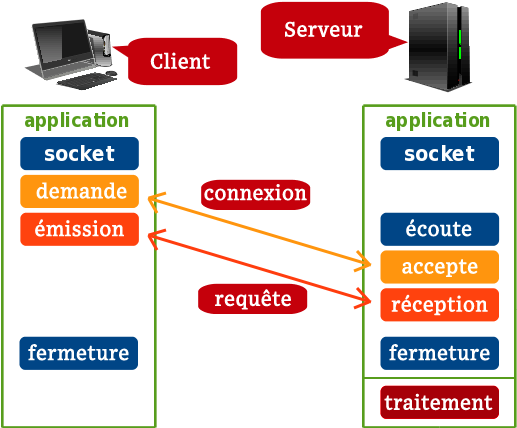
\includegraphics[height=150pt]{images/network/tcp-socket6.png}}
		\invisible{
			\begin{itemize}
				\item Dispose de classes prévues à cet effet en C\#
				\item Documentée en C\# par Microsoft
				\item Permet d'envoyer des octets, donc flexible
			\end{itemize}
		}
	\end{frame}
	\begin{frame}{Socket TCP}
		\centerline{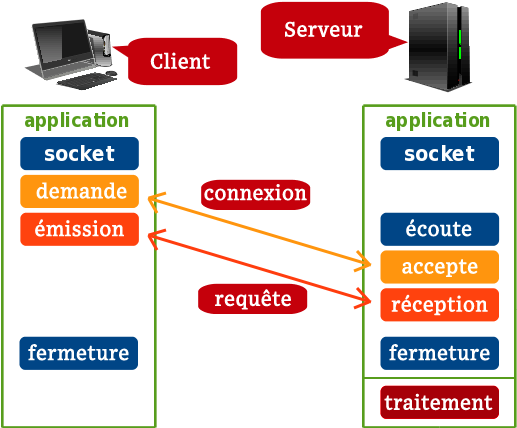
\includegraphics[height=150pt]{images/network/tcp-socket6.png}}
			\begin{itemize}
				\item Dispose de classes prévues à cet effet en C\# \pause
				\item Documentée en C\# par Microsoft \pause
				\item Permet d'envoyer des octets, donc flexible
			\end{itemize}
	\end{frame}
	
	\begin{frame}{Côté client}
		\centerline{\includegraphics<1>[height=140pt]{images/network/options.png}}
	\end{frame}
	
	\begin{frame}{Côté client}
		\centerline{\includegraphics<1>[height=140pt]{images/network/polandball_3D.png}}
	\end{frame}
	
	\begin{frame}{Résultat}
		\centerline{\includegraphics<1>[height=170pt]{images/network/server.png}}
	\end{frame}
	
	\section{Conclusion}
	
	\begin{frame}{Notre application}
		Voici une vidéo montrant un exemple d'utilisation de notre application :
		%vidéo -> présente les points clés de notre présentation
	\end{frame}
	
	\begin{frame}{Pour résumer}
		Nous avons fait une application Unity :
		\begin{itemize}
			\item Fonctionnant sur tablette Windows
			\item Utilisation simplifiée pour des utilisateurs novices via 
			\begin{itemize}
				\item Une palette de couleurs réduite
				\item Un placement de l'objet créé en 3 étapes
				\item Un système d'icônes clair
			\end{itemize}
			\item Un export de l'objet sur un serveur distant dans une scène
		\end{itemize}
	\end{frame}
		
\end{document}
